% !TeX encoding = UTF-8
% !TeX document-id = {856115b6-76ae-40a0-94c7-827233f04a27}
\documentclass[13pt,a4paper, listof=entryprefix, bibliography=totocnumbered,toc=listofnumbered,lof=listofnumbered]{scrartcl}
																			%toc=listofnumbered
% WICHTIG!!!
% Pseudokommentar um pdflatex zu erlauben andere Programme zu nutzen z.B. gnuplot
% !TeX TXS-program:compile = txs:///pdflatex/[--shell-escape] | txs:///makeindex | txs:///biber | txs:///pdflatex/[--shell-escape]

\usepackage[normalem]{ulem}
\usepackage[ngerman]{babel}
\usepackage{romannum}
\usepackage[utf8]{inputenc}

%Paket fuer einheitlichen Schriftsatz Times Roman
\usepackage{mathptmx}

%Paket wurde eingefügt, damit die Trennung auch bei Umlauten korrekt erfolgt
\usepackage[T1] {fontenc} 
%sollte ein Wort trotzdem mal nicht richtig getrennt werden, kann dies durch
%\hyphenation{Durch-füh-rung} %manuel getrennt werden.


\usepackage{amsmath}
\usepackage{booktabs}
\usepackage{nccmath}
\usepackage{amsfonts}
\usepackage{amssymb}
\usepackage{adjustbox}
\usepackage{graphicx}
\usepackage{fancyhdr}
\usepackage{array}
\usepackage{tabularx}
\usepackage{geometry}
\usepackage{setspace}
\usepackage[right]{eurosym}
\usepackage[printonlyused]{acronym}
\usepackage{subfig}
\usepackage{floatflt}
\usepackage[usenames,dvipsnames]{color}
\usepackage{colortbl}
\usepackage{xcolor}
\usepackage{paralist}
\usepackage{array}
%\usepackage{titlesec}
\usepackage{parskip}
\usepackage{picinpar}
\usepackage[pdfpagelabels=true]{hyperref}
\usepackage{listings}
\usepackage{csquotes}
\usepackage{url}
\usepackage{float}
\usepackage{pgfplots}
\usepackage[nonumberlist, nogroupskip]{glossaries}
\usepackage{eurosym}
\usepackage{textcomp}
 
\usepackage{ltablex}

\usepackage{lscape}
\usepackage{verbatim}
\usepackage{enumitem} 
\usepackage{tex/ampl}
\usepackage{multirow}
\setitemize{leftmargin=*}
%\usepackage{pdflscape}
\usepackage[miktex]{gnuplottex}
% Wird benötigt, damit die Tabelle beim Spaltentyp X die gesamte Seitenbreite verwendet. Ist unter anderem bei Tabellen in der Parameter definiert werden hilfreich.
\keepXColumns




%Wird zur Darstellung von Algorithmen benötigt
\usepackage{algorithm}
\usepackage{algorithmic}

\floatname{algorithm}{Algorithmus}
\floatname{List of Algorithms}{Algorithmen}
\captionsetup[algorithm]{justification=raggedright,singlelinecheck=false}

% Indizes
\index{Algorithmus -- Pseudocode}
\index{Optimierungsproblem -- Definition}


% Stichwortverzeichnis
\usepackage[nonewpage]{imakeidx}
\makeindex[intoc=false, title=, options=-g -s tex/_index \%.idx]


%-----------------------------------------------------------------------------------
% Bibilothek
%-----------------------------------------------------------------------------------
% Einbinden des BibLateX paketes mit Ausgabeeinstellungen							   
\usepackage[
style=alphabetic,          % Zitierstil
maxbibnames=50,            % alle Autorennamen anzeigen
maxcitenames=4,            % maximale Namen, die im Kürzel angezeigt werden
autocite=inline,           % regelt Aussehen für \autocite (inline=\parancite)
block=space,               % kleiner horizontaler Platz zwischen den Feldern
backref=false,             % Keine Angaben auf welchen Seiten die Quelle referenziert ist
% backrefstyle=three+,       % fasst Seiten zusammen, z.B. S. 2f, 6ff, 7-10
% date=short,                % Datumsformat
backend = biber,           % Backnend für Aufbereitung
doi=false,		%Keine Ausgabe des DOI
isbn=false		% Keine Ausbage der ISBN
]{biblatex}

%Doppelunkt nach Autorennamen
\renewcommand*{\labelnamepunct}{\addcolon\addspace}

%Zusätzliche für Umbrüche für Kleinbuchstaben z.B. in URLs
\appto\UrlBreaks{\do\a\do\b\do\c\do\d\do\e\do\f\do\g\do\h\do\i\do\j
	\do\k\do\l\do\m\do\n\do\o\do\p\do\q\do\r\do\s\do\t\do\u\do\v\do\w
	\do\x\do\y\do\z}



\newcounter{verzeichnis}
\setcounter{verzeichnis}{1}

%zur Verwendung von TikZ
\usepackage{tikz}
\usepackage{tikz-qtree, tikz-qtree-compat}
\usetikzlibrary{patterns}
%\usepackage[justification=RaggedRight,singlelinecheck=false]{caption}
\usetikzlibrary{positioning,calc}
\usetikzlibrary{snakes,arrows,shapes,automata,positioning}
\usetikzlibrary{decorations,decorations.pathmorphing,decorations.markings,trees,arrows}
\usetikzlibrary{shapes.geometric}
\usetikzlibrary{arrows.meta}
\usetikzlibrary{graphs,quotes,angles, babel}


%Abstände der Einträge
\setlength{\bibitemsep}{1em}     % Abstand zwischen den Literaturangaben
\setlength{\bibhang}{2em}        % Einzug nach jeweils erster Zeile

% Kürzel soll vier Buchstaben der Autoren enthalten statt drei
\DeclareLabelalphaTemplate{
	\labelelement{
		\field[final]{shorthand}
		\field{label}
		\field[strwidth=4,strside=left,ifnames=1]{labelname}
		\field[strwidth=2,strside=left,ifnames=2]{labelname}
		\field[strwidth=1,strside=left]{labelname}
	}
	\labelelement{
		\field[strwidth=2,strside=right]{year}
	}
}

% Bibliothek der Quellen
\bibliography{tex/biblatex.bib}
\label{bib}


% --------------------------------------------------------------------------------
% Einstellung für Listings
% --------------------------------------------------------------------------------
\lstset{basicstyle=\footnotesize, captionpos=b, breaklines=true, showstringspaces=false, tabsize=2, frame=lines, numbers=left, numberstyle=\tiny, xleftmargin=2em, framexleftmargin=2em}
\makeatletter
\def\l@lstlisting#1#2{\@dottedtocline{1}{0em}{1em}{\hspace{1,5em} Lst. #1}{#2}}
\makeatother

\makeatletter
\def\l@algorithm#1#2{\@dottedtocline{1}{0em}{0em}{\hspace{0em} Algorithmus #1}{#2}}
\makeatother

%Einstellung für Umlaute in Listings
\lstset{literate=%
    {Ö}{{\"O}}1
    {Ä}{{\"A}}1
    {Ü}{{\"U}}1
    {ß}{{\ss}}1
    {ü}{{\"u}}1
    {ä}{{\"a}}1
    {ö}{{\"o}}1
    {~}{{\textasciitilde}}1
}

%Einstellungen zur Vermeidung von Einrückung bei Aufzählungen
%Aufzählungen mit Punkten
\newenvironment{FHitemize}{\begin{list}{$\bullet$} {\leftmargin1.5em \labelsep1em \rightmargin0cm \parsep0.5ex plus0.2ex minus0.1ex \itemsep0ex plus0.2ex}}{\end{list}}
%Aufzählungen mit Nummerierungen
\setlist[enumerate]{wide=0pt, leftmargin=*}


% --------------------------------------------------------------------------------
% Seitenformate
% --------------------------------------------------------------------------------
%Seitenformat
%\geometry{a4paper, top=27mm, left=30mm, right=20mm, bottom=32mm, headsep=12mm, footskip=12mm}
 \geometry{a4paper, top=20mm, left=30mm, right=20mm, bottom=25mm, headsep= 8mm, footskip=12mm}

% --------------------------------------------------------------------------------
% Metainformationen
% --------------------------------------------------------------------------------
\hypersetup{unicode=false, pdftoolbar=true, pdfmenubar=true, pdffitwindow=false, pdfstartview={FitH},
	pdftitle={Vorlage},
	pdfauthor={Studierender},
	pdfsubject={Abschlussarbeit},
	pdfcreator={\LaTeX\ with package \flqq hyperref\frqq},
	pdfproducer={pdfTeX \the\pdftexversion.\pdftexrevision},
	pdfkeywords={Vorlage},
	pdfnewwindow=true,
	colorlinks=true,linkcolor=black,citecolor=black,filecolor=magenta,urlcolor=black}
\pdfinfo{/CreationDate (D:20141024101000)}
\pgfplotsset{compat=1.11}

%-----------------------------------------------------------------------------------
% Abkürzungen AKRONYME HIER ERGÄNZEN
%-----------------------------------------------------------------------------------
\glssetwidest{MLCLSP}% Längste Abkürzung für eine korrekte Einrückung

\makenoidxglossaries %Leeres Verzeichnis erstellen
%\makeglossaries %Leeres Verzeichnis erstellen

%Abkürzungen hinzufügen
\newacronym{LIP}{LIP}{Labor für Informationstechnik und Produktionslogistik}
\newacronym{OTH}{OTHR}{Ostbayerische Technische Hochschule Regensburg}
\newacronym{MRP}{MRP}{Material Requirements Planing}
\newacronym{RCPSP}{RCPSP}{Resource-Constrained Project Scheduling Problem}
\newacronym{MLCLSP}{MLCLSP}{Multi-level capacipated lot-sizing Problem}
\newacronym{ME}{ME}{Mengeneinheit}
\newacronym{ZE}{ZE}{Zeiteinheit}
\newacronym{GE}{GE}{Geldeinheit}
\newacronym{WIP}{WIP}{Work in process}
\newacronym{ILOG}{ILOG}{IBM ILOG CPLEX Optimisation Studio}
\newacronym{OPL}{OPL}{Open Programming Language}
\newacronym{PPS}{PPS}{Produktionsplanung- und Steuerung}
\newacronym{FIFO}{FIFO}{First in first out}
\newacronym{LIFO}{LIFO}{Last in first out}
\newacronym{DLZ}{DLZ}{Durchlaufzeit}
\newacronym{ERP}{ERP}{Enterprise-Resource-Planning}

\addtokomafont{disposition}{\boldmath}
%\addtokomafont{section}{\bfseries}


% !TEX root = ../Masterarbeit.tex

%Definition für \hline ohne Seitenumbruch
\makeatletter
\def\nobreakhline{%
	\noalign{\ifnum0=`}\fi
	\penalty\@M
	\futurelet\@let@token\LT@@nobreakhline}
\def\LT@@nobreakhline{%
	\ifx\@let@token\hline
	\global\let\@gtempa\@gobble
	\gdef\LT@sep{\penalty\@M\vskip\arrayrulewidth}% <-- change here
	\else
	\global\let\@gtempa\@empty
	\gdef\LT@sep{\penalty\@M\vskip-\arrayrulewidth}% <-- change here
	\fi
	\ifnum0=`{\fi}%
	\multispan\LT@cols
	\unskip\leaders\hrule\@height\arrayrulewidth\hfill\cr
	\noalign{\LT@sep}%
	\multispan\LT@cols
	\unskip\leaders\hrule\@height\arrayrulewidth\hfill\cr
	\noalign{\penalty\@M}%
	\@gtempa}
\makeatother

\begin{document}
	% --------------------------------------------------------------------------------
	% Globale Formateinstellungen
	% --------------------------------------------------------------------------------
	\onehalfspacing
	% Abstände Überschrift
%	\titlespacing{\section}{0pt}{42pt}{6pt}
%	\titlespacing{\subsection}{0pt}{12pt}{6pt}
%	\titlespacing{\subsubsection}{0pt}{12pt}{6pt}

	% Kopf- und Fußzeile
	\pagestyle{fancy}
	\lhead{}\chead{}
	\rhead{\thesection\space\contentsname}
	\lhead{}\cfoot{}
	\rfoot{\ \linebreak \thepage}
	\renewcommand{\headrulewidth}{0.4pt}
	\renewcommand{\footrulewidth}{0.4pt}

	% Nummerierung
	\renewcommand{\thesection}{\Roman{section}}
	\renewcommand{\theHsection}{\Roman{section}}
	\pagenumbering{Roman}

	% eigene Farbdefinitionen
	\definecolor{lip}{HTML}{3366FF}
	\definecolor{grey}{HTML}{ABABAB}

	\setkomafont{disposition}{\bfseries\normalsize} %für Times New Roman in Überschriften

\pagebreak
% !TEX root = ../0-Bachelorarbeit.tex

% ---------------------------------------------------------------------------
% Titelseite
% ---------------------------------------------------------------------------
\thispagestyle{empty}

	%LIP Schriftzug in eigener Farbe
\begin{singlespacing} 
    \textsf{\begin{minipage}{.4\textwidth} %Einbinden des Logos mit rechtsbündiger Ausrichtung. Weitere Logos im Bilderordner verfügbar.
            \begin{flushright}
                
\includegraphics[width=1\textwidth]{Bilder/OTH_IM_Logo}\\
            \end{flushright}
        \end{minipage}
        \begin{minipage}{.6\textwidth}
            \large
            \textcolor{lip}{\textbf{Labor für Informationstechnik und\\Produktionslogistik (LIP)}} %Farbe setzen
            \small
            \textbf{\\Verfahren, Strategien, Prozesse und IT-Systeme}
            \\Professor Dr. Frank Herrmann
        \end{minipage}
    }
\end{singlespacing} 
    % Zeilenabstand
    \onehalfspacing	
    
    %Beschriftung der Titelseite
    \begin{center}
        \vspace*{4cm} %4 cm Vorspann
        \Large
	    \textbf{Studienarbeit im Fach Data Mining}\\ %Titel der Arbeit
        \large
        \textbf{Analyse eines Affenpocken Datensatzes}\\ %Untertitel der Arbeit

        \vspace*{2cm} %2 cm Vorspann
        \textbf{Studienarbeit}\\ %Titel der Arbeit
        \vspace*{1cm}
    \large
        an der Fakultät Informatik und Mathematik\\
        im Studiengang Wirtschaftsinformatik
    \\ %Fakultät und Studiengang
    
    \vspace*{2cm} 
    \normalsize
        \begin{center}
            eingereicht\\
            im Januar 2023\\
        \textbf{Linus Schlepp}\\
        Almenstraße 23, 93142 Maxhütte-Haidhof
            
            
        \end{center}
        \vspace*{2cm}      
        \begin{table}[H]
            \centering
            \begin{tabular}{ll}
                Professor Dr. Edwin Schicker \\
              
            \end{tabular}%
        \end{table}%
        
        
        
    \end{center}
    
\pagebreak

\pagebreak

		% ------------------------------------------------------------------------------
		% Inhaltsverzeichnis
		% ------------------------------------------------------------------------------
		% Inhaltsverzeichnis
		\singlespacing %Zeilenabstand reduzieren
		\setcounter{section}{0}
		\setcounter{page}{1}
		\addcontentsline{toc}{section}{Inhaltsverzeichnis} %Hinzufügen des Inhaltsverzeichnises selbst

		\tableofcontents %Ausgabe des Inhaltsverzeichnisses
		\pagebreak

		% ------------------------------------------------------------------------------
		% Setzen der Nummerierungen für Normaltext
		% ------------------------------------------------------------------------------
		\onehalfspacing %Zeilenabstand auf 1.5
		\renewcommand{\thesection}{\arabic{section}} %Arabische Beschriftung für Absatznummern
		\pagenumbering{arabic}	%Seitennummerierung auf arabisch setzen
		\setcounter{page}{1}	%Seitenzahl für Inhalt auf 1 setzen
		\setcounter{section}{0}	% Kopfzeile mit aktuellem Hauptkapitel darstellen
		\renewcommand{\sectionmark}[1]{\markright{#1}}	%Section ausgeben
		\renewcommand{\subsectionmark}[1]{}				%Subsection nicht ausgeben
		\renewcommand{\subsubsectionmark}[1]{}			%Subsubsection nicht ausgeben
		\rhead{\rightmark}								%Ausgabe Rechtsbündig


	%------------------------------------------------------------------------------
	%	Inhalt
	%------------------------------------------------------------------------------

		%------------------------------------------------------------------------------
		%	Installation
		%------------------------------------------------------------------------------
	\section{Vorwort}
		\label{ch:vorwort}


	\section{Analyse der Daten}
		\label{ch:analyse_daten}

	In diesem Kapitel findet eine Analyse der vorliegenden Daten statt. Der Datensatz weißt insgesamt 25000 Zeilen und 11 Spalten auf, davon sind 
	neun Features, einer ist der Index und einer stellt die Ergebnis-Spalte dar. Damit Funktionen, wie \url{pandas.DataFrame.replace} und 
	\url{pandas.DataFrame.query} problemlos verwendet werden können, war es notwendig, die Leerzeichen in den Spaltenbennenungen mit Unterstrichen zu ersetzen. 
	So wurde beispielsweise \url{Systmic Illness} zu \url{Systemic_Illness}.  Die Spalte \url{Patient_ID} wurde als Index verwendet. 
	\url{MonkeyPox} stellt die Ergebnis-Spalte dar. Das folgende Bild zeigt die Aufteilung der Spalten und die korrespondierenden Werte:

	\begin{figure}[H]
		\centering
		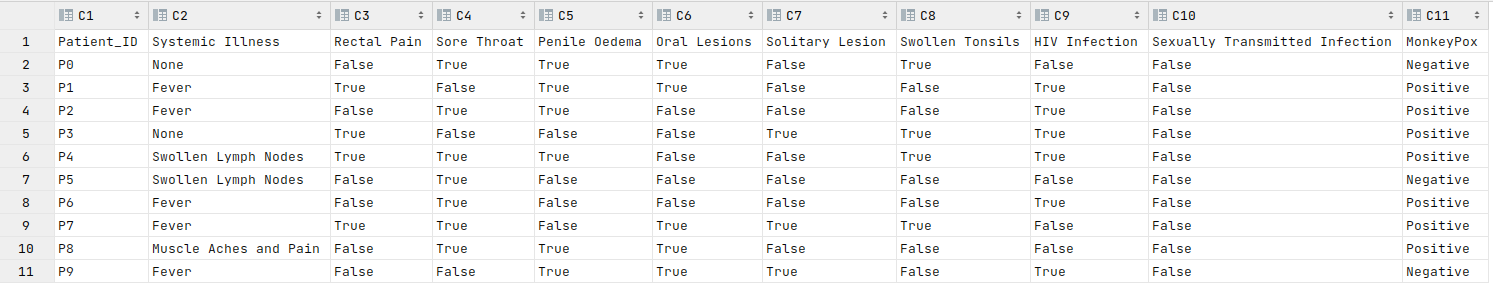
\includegraphics[width=0.8\linewidth]{Bilder/data_table.png}
		\captionof{figure}[Ausschnitt aus dem vorliegendem Datensatz]{Ausschnitt aus dem vorliegendem Datensatz}
		\label{fig:data_table}
	\end{figure}

	Bei den Werten der Features handelt es sich zu einem großen Teil, um \url{bool} Werte. Die Spalte \url{Systemic Illness}, stellt dabei eine Ausnahme dar. In dieser werden
	vier \url{str} Werte verwendet: \url{None}, \url{Fever}, \url{Swollen Lymph Nodes} und \url{Muscel Aches and Pain} in \url{int} Werte umgewandelt. So wurde \url{None} zu 1,
	\url{Fever} zu 2, \url{Swollen Lymph Nodes} zu 3 und \url{Muscle Aches and Pain} zu 4. Die Spalte \url{MonkeyPox} enthält die Werte \url{Positive} und \url{Negative} und gibt
	an, ob der entsprechende Patient an Affenpocken erkrankt ist.

	Die Werteverteilung der Features, welche \url{bool} Werte enhalten, ist in dieser Tabelle aufgelistet: 
	
	\begin{table}[H]
		\centering
		\begin{tabular}{|l|l|l|l|l|l|l|l|}
			\hline  & \url{RectalPain}&  \url{SoreThroat}	& \url{PenileOedema} & \url{OralLesion} & \url{SolitaryLesion} &\url{SwollenTonsils} & \url{HIVInfection} \\
			\hline True & 12345 & 12554 & 12612 & 12486 & 12527 & 12533 & 12584   \\
			\hline False & 12655 & 12446 & 12388& 12514 & 12473 & 12467 & 12416 \\
			\hline
		\end{tabular}
		\caption{Werteverteilung der verschiedenen Features} %Hinzufügen einer Tabellenbeschriftung
		\label{tab:werteverteilung_features}
	\end{table}

	Es lässt sich feststellen, dass die Werteverteilung innerhalb der \url{bool} Features sehr gleichmäßig ist. 
	In Bezug auf die \url{str} Feature (\url{SystemicIllness}) lässt sich die Wertevereilung, durch dieses Diagramm
	visualisieren: 

	\begin{figure}[H]
		\centering
		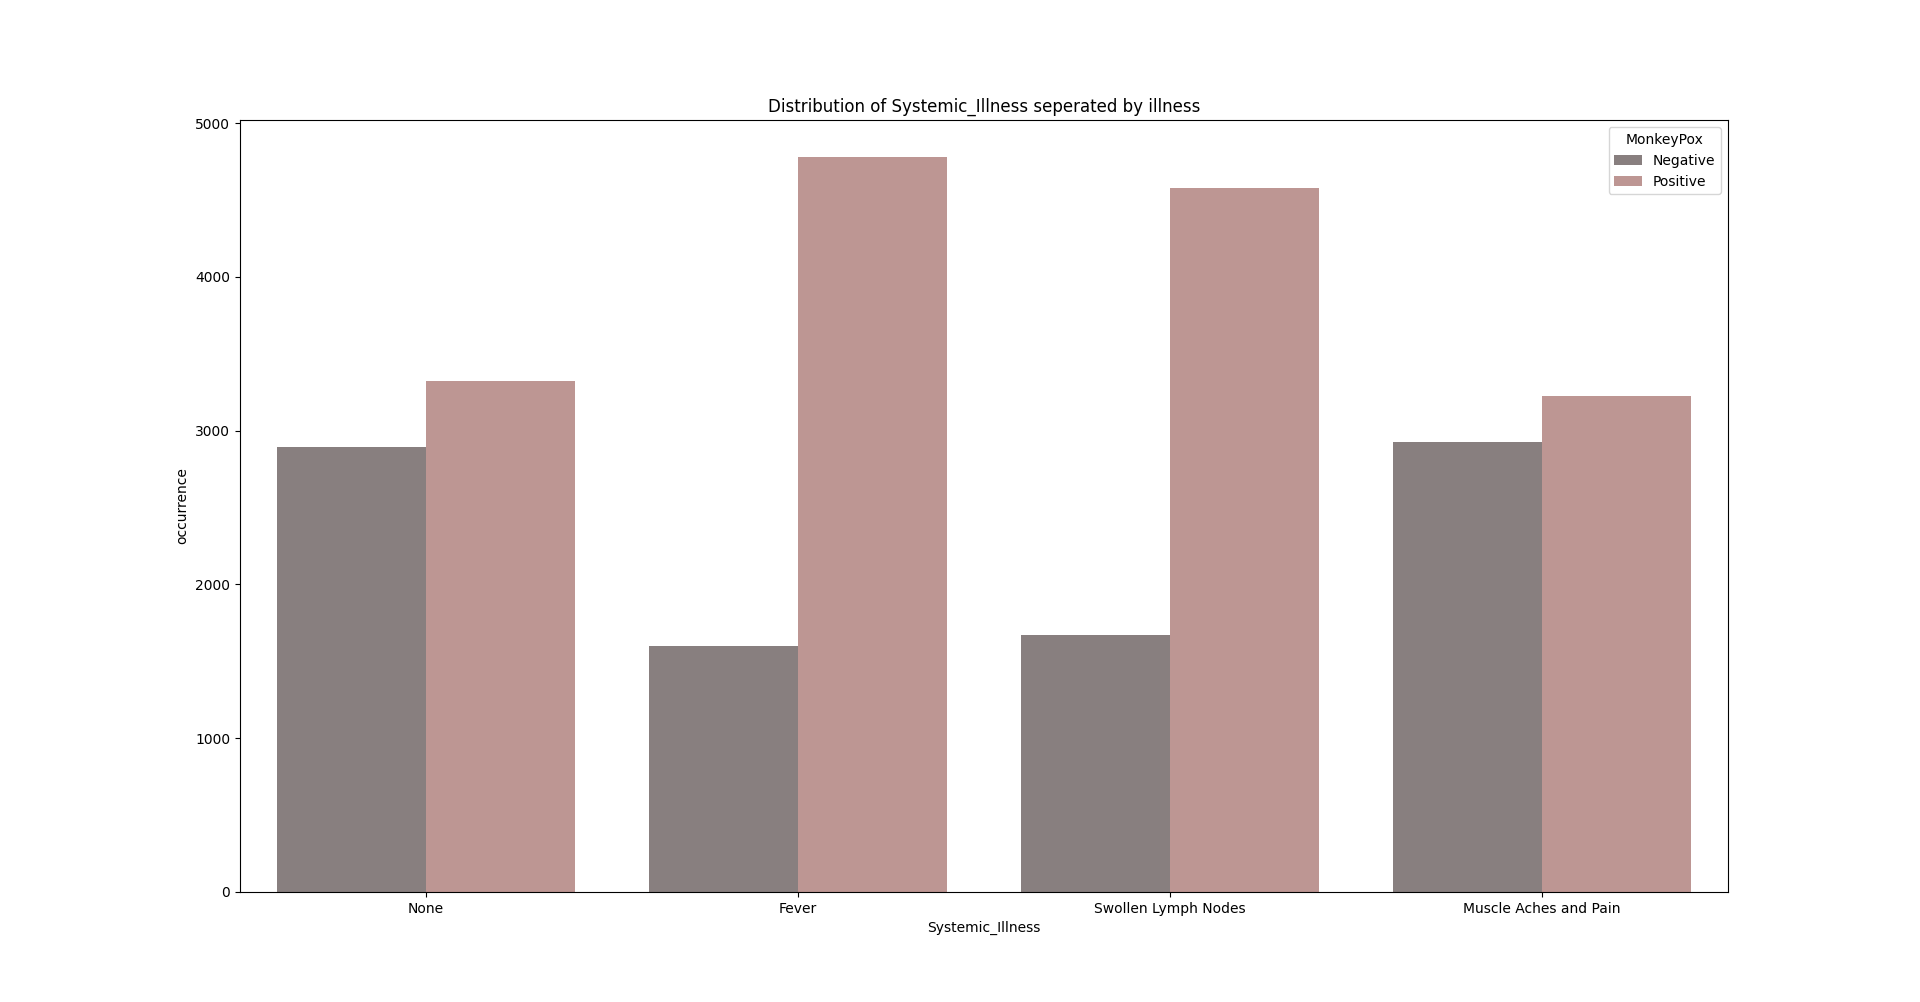
\includegraphics[width=0.8\linewidth]{Bilder/systemic_illness_plot.png}
		\captionof{figure}[Werteverteilung des Feature \url{SystemicIllness}]{Werteverteilung des Feature \url{SystemicIllness}}
		\label{fig:systemic_illness_plot}
	\end{figure}

	In Betracht auf auf Spalte \url{MonkeyPox} lässt sich sagen, dass 15909 Patienten an Affenpocken erkrankt sind, während 9091 \url{Negative} sind,
	also nicht Affenpocken erkrankt sind. 

	

	\subsection{Visuelle Analyse}
		\label{ch:visuelle_analyse}

	Zur visuellen Analyse der Daten wurden zum großen Teil, Balkendiagramme verwendet. 

	

		\pagebreak
		%-------------------------------------------------------------------------------------
		% Verzeichnisse %-------------------------------------------------------------------------------------
		\rhead{Verzeichnisse} %Kopftextbeschriftung

		\stepcounter{section}
		\phantomsection \label{Verzeichnisse}
		\addcontentsline{toc}{section}{Verzeichnisse} %Ohne Nummer ins Inhaltsverzeichnis
		\renewcommand{\thesection}{\Roman{verzeichnis}}
		\section*{Verzeichnisse}
		% Literaturverzeichnis
		\rhead{Verzeichnisse}
   		\phantomsection \label{Literaturverzeichnis}
		\renewcommand{\refname}{Literaturverzeichnis}
		\printbibliography
		\pagebreak

		% Abbildungsverzeichnis
		\stepcounter{verzeichnis}
		\listoffigures
		\pagebreak

		% Tabellenverzeichnis

		\stepcounter{verzeichnis}
		\listoftables
		\pagebreak

        % Listingverzeichnis
        \stepcounter{verzeichnis}
        \lstlistoflistings
        \pagebreak

        % Algorithmusverzeichnis
        %\renewcommand{\listalgorithmname}{Algorithmenverzeichnis}
        %\listofalgorithms
        \stepcounter{verzeichnis}

        \section{Algorithmenverzeichnis}
        \vspace{-2em}
        \listoftoc[]{loa}



% Stichwortverzeichnis
\pagebreak
\stepcounter{verzeichnis}
% Stichwortverzeichnis soll im Inhaltsverzeichnis auftauchen
\section{Stichwortverzeichnis}

% Abstand analog der anderen Verzeichnisse reduzieren
\vspace{-3em}

% Stichwortverzeichnis endgueltig anzeigen

\printindex

		% Abkürzungen
        \pagebreak
		\stepcounter{verzeichnis}
		\section{Abkürzungsverzeichnis}
		\vspace{-4em} % Abstand analog der anderen Verzeichnisse reduzieren
		\printnoidxglossary[type=\acronymtype,style=alttree,title=,toctitle=] %automatischen Titel und Gliederungsbeschriftung unterdrücken - sonst steht da Glossarie
		%\printglossary[type=\acronymtype,style=alttree,title=,toctitle=] %automatischen Titel und Gliederungsbeschriftung unterdrücken - sonst steht da Glossarie
		\newpage

		% % ---------------------------------------------------------------------------------
		% % Anhang
		% % ---------------------------------------------------------------------------------
		\rhead{Anhang}        %Kopftextbeschriftung
		\begin{appendix}
			\phantomsection \label{Anhang}
			\section*{Anhang}\addcontentsline{toc}{section}{Anhang} %Anhang ohne Nummer
			\renewcommand{\thesection}{\Roman{section}}

			\setcounter{section}{0} %Counter für Nummerierung der Anhänge initalisieren
			\section{Remotenutzung der CIP-Pool-Rechner}
			\label{app:remotenutzung}
			Für die Remotenutzung der CIP-Pool-Rechner sind folgende Schritte zu vollziehen. \\
			Es sei angemerkt, dass nach aktuellem Stand (09.12.2020) die CIP-Pool-Rechner bis März 2021 zur Remotenutzung zur Verfügung stehen.
			
			\begin{enumerate}
				\item Eine Verbindung mit dem Hochschulnetz muss aufgebaut werden. Dies ist mittels VPN (siehe \href{https://www.oth-regensburg.de/supportwiki/doku.php?id=public:netz:vpn-forticlient}{\underline{Anleitung}}) möglich.
				
				\item Die Seite \url{https://remote-cip-wa.hs-regensburg.de/RDWeb/} muss aufgerufen werden. \\
				Im Anschluss muss die Anmeldung mittels NDS-Kennung im Format \textbf{HSR\textbackslash}abc12345 erfolgen.
				
					% \begin{figure}[H]
      				% \centering
        			% \includegraphics[width=1\textwidth]{Bilder/201209_Remote1}
        			% \caption{CIP-Pool-Remotenutzung: Anmeldung auf Website}
        			% \label{fig:201209_Remote1}
        			% \end{figure}				
				\smallskip
				\item Nach erfolgter Anmeldung ist durch einen Mausklick der CIP-Pool auszuwählen, dessen Rechner man nutzen möchte. In dieser Anleitung wird der CIP-Pool der Maschinenbau-Fakultät ausgewählt.
				
					% \begin{figure}[H]
      				% \centering
        			% \includegraphics[width=1\textwidth]{Bilder/201209_Remote2}
        			% \caption{CIP-Pool-Remotenutzung: Auswahl des CIP-Pools}
        			% \label{fig:201209_Remote2}
        			% \end{figure}
				
				\item Die aufkommende Meldung ist zu bestätigen. Es wird ein Öffnen mit der Standardanwendung empfohlen.

					% \begin{figure}[H]
      				% \centering
        			% \includegraphics[width=1\textwidth]{Bilder/201209_Remote3}
        			% \caption{CIP-Pool-Remotenutzung: Öffnen der Anwendung zur Remote Desktop Connection}
        			% \label{fig:201209_Remote3}
        			% \end{figure}				
				\medskip
				\item Die aufkommende Meldung ist durch Klicken auf \glqq Verbinden\grqq{} zu bestätigen.

					% \begin{figure}[H]
      				% \centering
        			% \includegraphics[width=1\textwidth]{Bilder/201209_Remote4}
        			% \caption{CIP-Pool-Remotenutzung: Bestätigen der Verbindung}
        			% \label{fig:201209_Remote4}
        			% \end{figure}				
				
				\item Bevor der CIP-Rechner nun genutzt werden kann, muss erneut eine Anmeldung mittels NDS-Kennung im Format \textbf{HSR\textbackslash}abc12345 erfolgen.
				
					% \begin{figure}[H]
      				% \centering
        			% \includegraphics[height=0.3\textheight]{Bilder/201209_Remote5}
        			% \caption{CIP-Pool-Remotenutzung: erneute Anmeldung}
        			% \label{fig:201209_Remote5}
        			% \end{figure}				
				\medskip
				\item Wenn der CIP-Rechner nicht mehr benötigt wird, ist eine Abmeldung des Benutzers durchzuführen.
				
					% \begin{figure}[H]
      				% \centering
        			% \includegraphics[width=1\textwidth]{Bilder/201209_Remote6}
        			% \caption{CIP-Pool-Remotenutzung: Abmeldung des Benutzers}
        			% \label{fig:201209_Remote6}
        			% \end{figure}				
				
			\end{enumerate}	
			
			
		\end{appendix}
    
\pagebreak
\rhead{Ehrenwörtliche Erklärung}

\phantomsection \label{Ehrenwörtliche Erklärung}
\pagenumbering{gobble}% Seitennummerierungsstil ganz ohne Ausgabe der Nummern verwenden!
\addcontentsline{toc}{section}{Ehrenwörtliche Erklärung} %Anhang ohne Nummer
%\section*{Ehrenwörtliche Erklärung}
\renewcommand{\thesection}{\Roman{section}}

\begin{singlespacing} 
    \textsf{\begin{minipage}{.4\textwidth} %Einbinden des Logos mit rechtsbündiger Ausrichtung. Weitere Logos im Bilderordner verfügbar.
            \begin{flushleft}
                \includegraphics[width=1.5\textwidth]{Bilder/OTH_Regensburg_Logo_3line_pos_bg}\\
            \end{flushleft}
        \end{minipage}
    }
\end{singlespacing} 
    % Zeilenabstand
    \onehalfspacing	
    
    %Beschriftung der Titelseite
    \begin{center}
        \vspace*{2 cm} %3 cm Vorspann
        \Large
        \textbf{ERKLÄRUNG \\ZUR MASTERARBEIT VON}
    \end{center}
        
	 \vspace*{1 cm} 
        \normalsize
        
	 \begin{table}[H]
        \begin{tabular}{ll}
        Name: & N a m e \\
        Vorname: & V o r n a m e \\
        Studiengang: & Informatik (M.Sc.)
        \end{tabular}
    \end{table}
    
     \vspace*{1 cm} 
        \normalsize
    

    \begin{enumerate}
        \item Mir ist bekannt, dass dieses Exemplar der Masterarbeit als Prüfungsleistung in das Eigentum der Ostbayerischen Technischen Hochschule Regensburg übergeht.\\
        
        \item Ich erkläre hiermit, dass ich diese Masterarbeit selbständig verfasst, noch nicht anderweitig für Prüfungszwecke vorgelegt, keine anderen als die angegebenen Quellen und Hilfsmittel benutzt sowie wörtliche und sinngemäße Zitate als solche gekennzeichnet habe. 
    \end{enumerate}


     \vspace*{3 cm} 
        \normalsize
        
    
    Regensburg, den TT.MM.JJJJ\\ \\
....................................................\\
Unterschrift

	\end{document}
